\section{Robot Kinematics and Dynamics}

\subsection{Locate the robot and the objects in the scene}

Here we introduce a fundamental question in robot kinematics: how to describe the relative position and orientation of objects in a robotic environment. In particular, we are asked to determine spatial relationships between different elements in the scene, such as the robot arm, its base, the mobile platform, the conveyor belt, and the boxes.

The key questions are:

\begin{itemize}
  \item Where is the tool with respect to the base of the robot arm?
  \item Where is the mobile robot with respect to the base of the arm?
  \item Where is the box with respect to the mobile robot?
  \item Where is the conveyor belt with respect to the robot?
\end{itemize}

These questions are essential in defining the \textbf{coordinate frames} for each object and in understanding \textbf{how to transform} positions and orientations from one frame to another using homogeneous transformations. This is a prerequisite for solving forward and inverse kinematics problems, motion planning, and control.

\hfill

\subsection{Where is the part of interest of the robot?}

The key kinematic problem in robotics is: \textbf{how to describe the position and orientation of a part of the robot (e.g., end-effector, mobile base) with respect to a desired reference frame}.

This is essential because robot control, planning, and coordination rely on being able to mathematically describe “where” a certain component of the robot is located. Typical examples of parts of interest include:
\begin{itemize}
  \item the end-effector of a manipulator,
  \item the mobile base of an autonomous robot.
\end{itemize}

\textbf{Kinematics of the robot} is therefore:
\begin{itemize}
  \item A fundamental problem for understanding how to use a robot;
  \item A problem that needs a clear and sound mathematical formalization.
\end{itemize}

The solution to this problem relies on the use of \textbf{reference frames}, often attached to relevant parts of the robot or to the environment. The \textbf{Body Frame} is the coordinate system fixed to the robot itself (e.g., at the base of a mobile platform or at a specific link of a manipulator). It moves with the robot and is used to express its configuration.

The diagram illustrates this idea: the robot's body frame (local frame) is shown inside a global reference frame (e.g., the room or map). The position and orientation of the body frame with respect to the global frame define the robot's pose.

\begin{figure}[H]
  \centering
  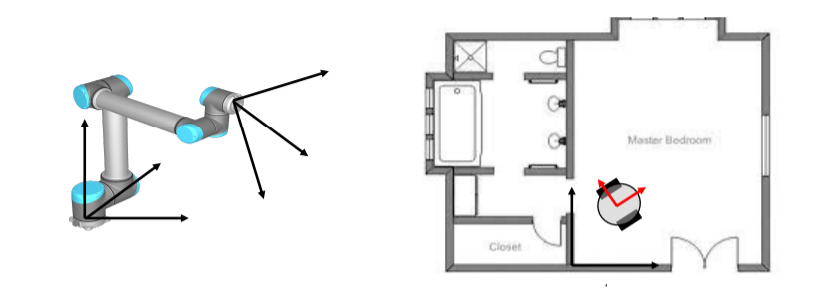
\includegraphics[width=\linewidth]{imgs/part_of_interest_kinematics.png}
  \caption{The robot’s body frame in a global environment frame.}
\end{figure}

\hfill

\subsection{Rigid Body Kinematics}

To analyze and control a robot, we must understand the kinematics of its components. Since a robot is composed of a sequence of rigid bodies (e.g., links in a manipulator), we must study the motion of rigid bodies to address robot kinematics properly.

\textbf{Key concepts:}
\begin{itemize}
  \item A robot is made up of one or more rigid bodies connected by joints.
  \item Understanding robot kinematics requires first understanding \textbf{rigid body kinematics}.
  \item The mathematical tools developed for rigid body motion — such as coordinate transformations and rotation matrices — are essential for solving robot kinematics.
\end{itemize}

The central question remains the same: \textit{"How can we describe the position and orientation of a rigid body with respect to a desired reference frame?"} This question is foundational and guides the development of the entire kinematic model of the robot.

To describe the position of objects in space, we use an \textbf{orthonormal reference frame} $F$, composed of three mutually orthogonal unit vectors (versors) $\hat{x}, \hat{y}, \hat{z}$, which define the orientation of the axes and intersect at an origin $O$.

\begin{itemize}
  \item Each versor defines the direction of an axis:
    \[
    \hat{x} = \begin{pmatrix}1 \\ 0 \\ 0\end{pmatrix}, \quad
    \hat{y} = \begin{pmatrix}0 \\ 1 \\ 0\end{pmatrix}, \quad
    \hat{z} = \begin{pmatrix}0 \\ 0 \\ 1\end{pmatrix}
    \]
  \item These versors form the basis of the frame $F$.
  \item A point $P$ in space can be located with respect to the frame $F$ using its coordinates $(x_P, y_P, z_P)$, and expressed as:
    \[
    \vec{OP} = x_P \hat{x} + y_P \hat{y} + z_P \hat{z}
    \]
    or in vector form:
    \[
    \vec{OP} = 
    \begin{pmatrix}
    x_P \\
    y_P \\
    z_P
    \end{pmatrix}
    \]
\end{itemize}

This formulation is the foundation for describing positions and motions in robotics, where the robot and its components are modeled as rigid bodies referenced to such frames.

\begin{figure}[H]
  \centering
  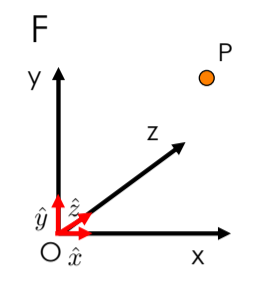
\includegraphics[width=0.3\linewidth]{imgs/rigid_body_reference_frame.png}
  \caption{Orthonormal reference frame $F$ and position vector of point $P$.}
\end{figure}

\hfill

\paragraph{Multiple Frames} \hfill

In robotic systems, it is common to use multiple coordinate frames to describe the positions of objects or parts of the robot. Each frame may be attached to a different body or component (e.g., base, end-effector, sensor).

\begin{itemize}
  \item Let $F_1$ and $F_2$ be two different reference frames.
  \item A point $P$ in space can be represented in both frames:
    \begin{itemize}
      \item $^1P$: coordinates of $P$ expressed in frame $F_1$.
      \item $^2P$: coordinates of $P$ expressed in frame $F_2$.
    \end{itemize}
  \item \textbf{In general,} the coordinate vectors $^1P$ and $^2P$ are different, because they are expressed with respect to different axes and origins.
\end{itemize}

To convert between representations in different frames, we use \textbf{coordinate transformations}, typically involving rotation and translation operations.

\begin{figure}[H]
  \centering
  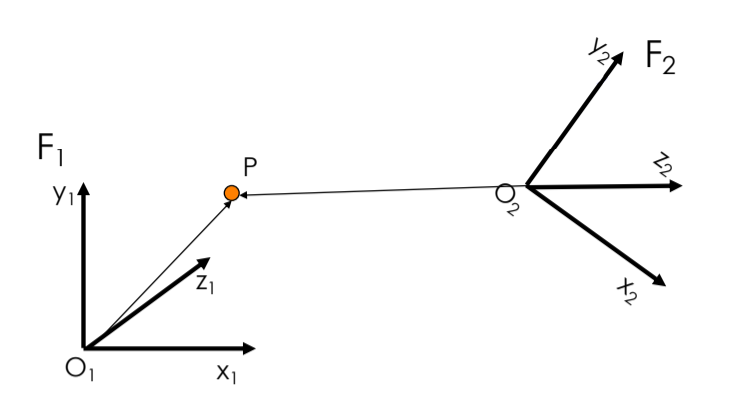
\includegraphics[width=0.65\linewidth]{imgs/multiple_frames.png}
  \caption{A point $P$ described in two different reference frames: $F_1$ and $F_2$.}
\end{figure}

\hfill

\paragraph{Pose and Body Frame} \hfill

A \textbf{rigid body} is defined as an object made up of a set of points that maintain a constant relative position. This implies that the body does not deform.

To describe a rigid body in space, we define its \textbf{pose}, which includes:
\begin{itemize}
  \item \textbf{Position}: the location of a point (usually the origin of the body frame) in a reference frame.
  \item \textbf{Orientation}: the angular configuration of the body frame with respect to the reference frame.
\end{itemize}

The pose of a rigid body is fully described by the pose of a frame rigidly attached to it, called the \textbf{body frame} ($F_B$).

\begin{itemize}
  \item The body frame moves with the rigid body.
  \item Its origin $O_B$ and axes $(x_B, y_B, z_B)$ define the configuration of the rigid body.
  \item The pose of the rigid body is defined with respect to a fixed reference frame, such as $F_0$.
\end{itemize}

\begin{figure}[H]
  \centering
  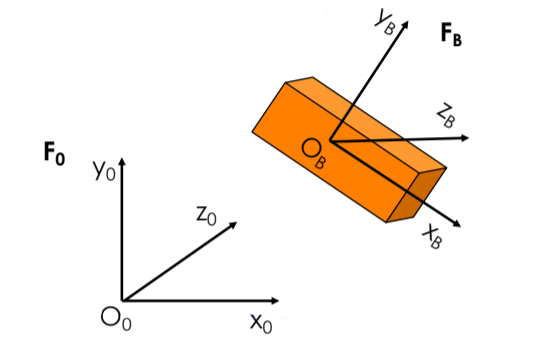
\includegraphics[width=0.6\linewidth]{imgs/pose_body_frame.png}
  \caption{Pose of a rigid body defined by the position and orientation of its body frame $F_B$ with respect to the reference frame $F_0$.}
\end{figure}

\hfill

\paragraph{Relative Position} \hfill

The \textbf{position} of a rigid body $B$ with respect to a fixed reference frame $F_0$ is defined by the position of the origin $O_B$ of the body frame $F_B$ relative to the origin $O_0$ of $F_0$.

\begin{itemize}
  \item This position is represented by the vector ${}^0\mathbf{O}_B$, which gives the coordinates of $O_B$ in frame $F_0$.
  \item It is written as:
    \[
    {}^0\mathbf{O}_B = 
    \begin{pmatrix}
      {}^0 O_{Bx} \\
      {}^0 O_{By} \\
      {}^0 O_{Bz}
    \end{pmatrix}
    =
    {}^0 O_{Bx} \hat{x}_0 + {}^0 O_{By} \hat{y}_0 + {}^0 O_{Bz} \hat{z}_0
    \]
  \item This vector describes the \textbf{relative position} of the body frame $F_B$ in the fixed frame $F_0$.
\end{itemize}

\begin{figure}[H]
  \centering
  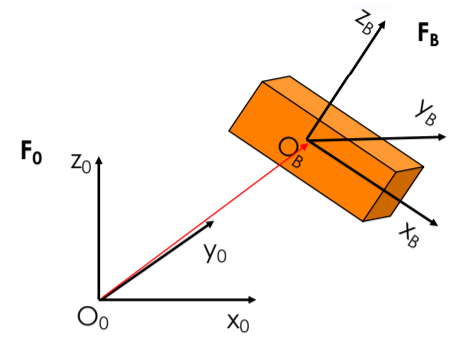
\includegraphics[width=0.5\linewidth]{imgs/relative_position.png}
  \caption{Relative position of the body frame $F_B$ with respect to the fixed frame $F_0$.}
\end{figure}

\hfill

\paragraph{Relative Orientation} \hfill

The orientation of a rigid body frame $F_B$ with respect to a reference frame $F_0$ can be described using different mathematical tools. The most common are:

\textbf{Rotation Matrix}:
\begin{itemize}
  \item The orientation of $F_B$ with respect to $F_0$ is given by the rotation matrix ${}^0R_B \in SO(3)$.
  \item The inverse orientation (from $F_0$ to $F_B$) is given by the transpose:
  \[
  {}^B R_0 = ({}^0 R_B)^T
  \]
  \item Rotation matrices can be composed via matrix multiplication:
  \[
  R_{AC} = R_{AB} \cdot R_{BC}
  \]
\end{itemize}

\textbf{Euler Angles}:
\begin{itemize}
  \item Represent orientation using three sequential angles: $(\rho, \vartheta, \varphi)$.
  \item These angles express rotations around selected axes (e.g., ZYX or XYZ convention).
  \item Euler angles are intuitive but suffer from singularities (gimbal lock).
\end{itemize}

\textbf{Unit Quaternions}:
\begin{itemize}
  \item A compact and non-singular representation of orientation.
  \item Useful for interpolation (e.g., SLERP) and for avoiding gimbal lock.
  \item Quaternions use a four-element vector and can be composed using quaternion algebra.
\end{itemize}

\begin{figure}[H]
  \centering
  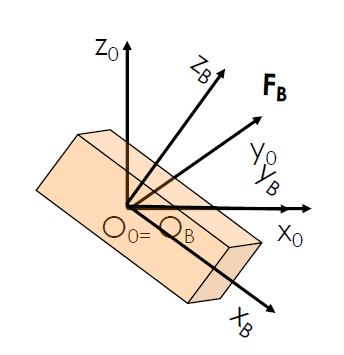
\includegraphics[width=0.4\linewidth]{imgs/relative_orientation.png}
  \caption{Orientation of frame $F_B$ with respect to $F_0$: axes are rotated but origins coincide.}
\end{figure}

\hfill

\paragraph{Homogeneous Transformations} \hfill

The \textbf{pose} of a rigid body with respect to a reference frame $F_0$ is defined by the pose of a frame $F_B$ rigidly attached to the body.

This pose is determined by two components:

\begin{itemize}
  \item \textbf{Position:} the relative translation of the origin $O_B$ of frame $F_B$ with respect to the origin $O_0$ of the reference frame $F_0$, expressed as a vector ${}^0\mathbf{O}_B$.
  \item \textbf{Orientation:} the relative orientation of the frame $F_B$ with respect to $F_0$, represented by the rotation matrix ${}^0R_B$.
\end{itemize}

Together, these two elements fully define the pose of the rigid body and can be compactly expressed using a \textbf{homogeneous transformation matrix} — which will be introduced and detailed in the following slides.

\begin{figure}[H]
  \centering
  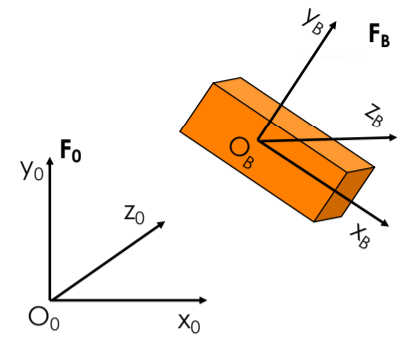
\includegraphics[width=0.4\linewidth]{imgs/homogeneous_transformations.png}
  \caption{The pose of the body frame $F_B$ with respect to the reference frame $F_0$ includes both translation and rotation.}
\end{figure}

To express both the position and orientation of a frame $F_1$ with respect to another frame $F_0$, we introduce the concept of a \textbf{homogeneous transformation}.

Consider a point $P$ expressed in frame $F_1$. Its coordinates in frame $F_0$ are given by:
\[
{}^0\!p = {}^0\!O_1 + {}^0\!R_1\, {}^1\!p
\]
This combines a translation (${ }^0\!O_1$) and a rotation (${ }^0\!R_1$). To make this operation more compact and composable, we adopt \textbf{homogeneous coordinates}.

\textbf{Homogeneous coordinates:}
\[
\tilde{p} = 
\begin{pmatrix}
p \\
1
\end{pmatrix}
\quad \text{(4x1 vector)}
\]

\textbf{Homogeneous transformation matrix:}
\[
{}^0\!T_1 =
\begin{pmatrix}
{}^0\!R_1 & {}^0\!O_1 \\
\mathbf{0} & 1
\end{pmatrix}
\quad \text{(4x4 matrix)}
\]

\textbf{Transformation of a point:}
\[
{}^0\!\tilde{p} = {}^0\!T_1\, {}^1\!\tilde{p}
\]

This matrix $T \in SE(3)$ (Special Euclidean group) allows us to perform roto-translations using a single matrix multiplication. The last row is always $\begin{pmatrix} 0 & 0 & 0 & 1 \end{pmatrix}$.

\begin{figure}[H]
  \centering
  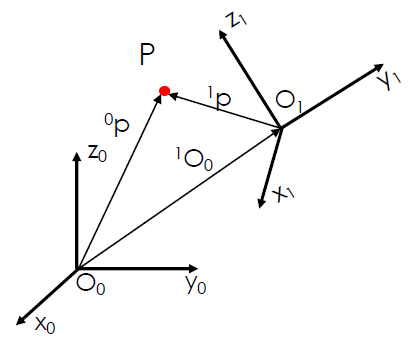
\includegraphics[width=0.5\linewidth]{imgs/homogeneous_point_position.png}
  \caption{Homogeneous transformation of a point $\tilde{p}$ from frame $F_1$ to frame $F_0$.}
\end{figure}

\textbf{Invertibility:}
The transformation matrix is always invertible. Its inverse is:
\[
{}^1\!T_0 =
\begin{pmatrix}
{}^1\!R_0 & -{}^1\!R_0\,{}^0\!O_1 \\
\mathbf{0} & 1
\end{pmatrix}
\]

This allows us to compute the pose of $F_0$ with respect to $F_1$ if the opposite is known.

\textbf{Composition of Transformations:}
Homogeneous transformations can be composed:
\[
{}^0\!T_2 = {}^0\!T_1\, {}^1\!T_2
\]
\[
{}^0\!\tilde{p} = {}^0\!T_2\, {}^2\!\tilde{p} = {}^0\!T_1\, {}^1\!T_2\, {}^2\!\tilde{p}
\]

This means that chains of transformations can be applied through successive matrix multiplications.

\begin{figure}[H]
  \centering
  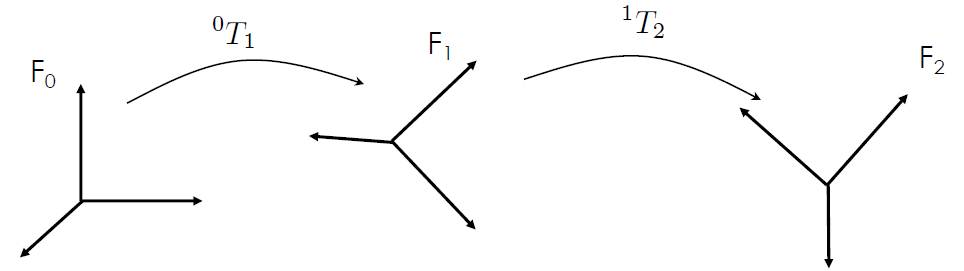
\includegraphics[width=\linewidth]{imgs/homogeneous_chain_composition.png}
  \caption{Composing transformations between multiple frames: $F_0 \rightarrow F_1 \rightarrow F_2$.}
\end{figure}

\hfill

\subsection{Homogeneous Transformations in Robotics}

Homogeneous transformations are widely used in robotics to describe the pose of robots and objects with respect to:
\begin{itemize}
  \item a fixed reference frame;
  \item neighboring or connected frames.
\end{itemize}

For example, consider a set of mobile robots each associated with a local frame $F_i$. Their pose with respect to a global frame $F_0$ is expressed by ${}^0T_i$, while their relative pose with respect to neighbors is expressed by transformations like ${}^1T_2$ or ${}^1T_3$.

\begin{figure}[H]
  \centering
  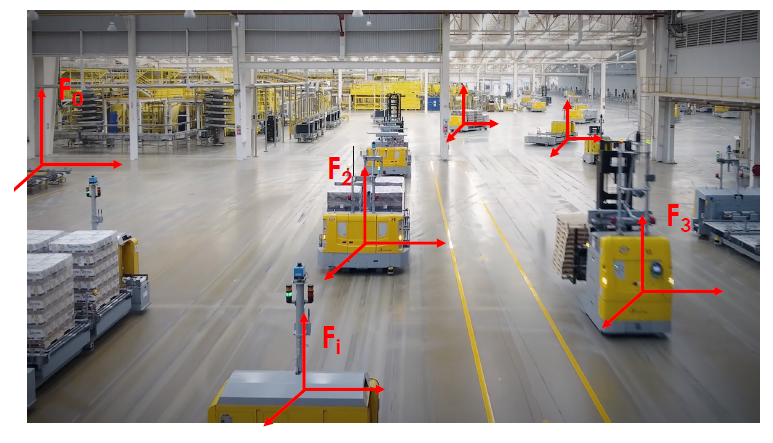
\includegraphics[width=0.75\linewidth]{imgs/homogeneous_robots_scene.png}
  \caption{Homogeneous transformations for multiple mobile robots.}
\end{figure}

The pose of the robot depends on the \textbf{configuration variables}, such as position $(x, y)$ and orientation $\vartheta$, and thus the homogeneous transformation matrix is:
\[
{}^0T_1 = \begin{pmatrix}
\cos\vartheta & -\sin\vartheta & 0 & x \\
\sin\vartheta & \cos\vartheta  & 0 & y \\
0 & 0 & 1 & 0 \\
0 & 0 & 0 & 1
\end{pmatrix}
\]

\begin{figure}[H]
  \centering
  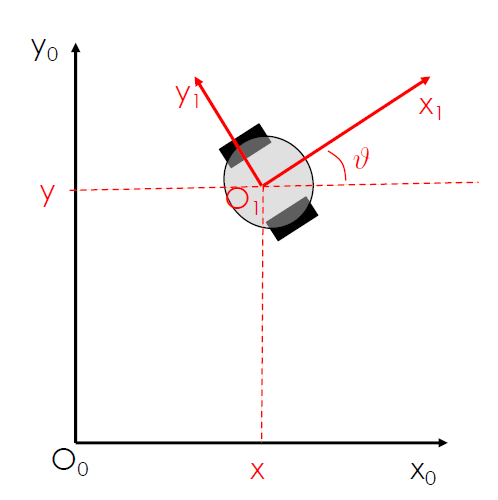
\includegraphics[width=0.45\linewidth]{imgs/homogeneous_planar_robot.png}
  \caption{Planar transformation of a wheeled mobile robot.}
\end{figure}

\paragraph{Planar robots:}
For wheeled mobile robots that move on a plane, the third row and third column of the matrix are always constant. Hence, we often reduce the transformation to a planar case:
\[
{}^0T_1 = \begin{pmatrix}
\cos\vartheta & -\sin\vartheta & x \\
\sin\vartheta & \cos\vartheta & y \\
0 & 0 & 1
\end{pmatrix}
\quad\text{with } {}^0R_1 \in SO(2), \quad {}^0O_1 \in \mathbb{R}^2
\]

\paragraph{Application in workspace:}
Homogeneous transformations are essential to relate different components of a robotic system:
\begin{itemize}
  \item ${}^0T_h$: hand with respect to robot base
  \item ${}^hT_{ob}$: object with respect to the hand
  \item ${}^0T_c$: camera with respect to the base
\end{itemize}

Using these matrices, one can map positions between components. For example, to express a point $p$ observed by a camera in the robot base frame:
\[
{}^0p = {}^0T_c \cdot {}^c p \qquad \forall p
\]

\begin{figure}[H]
  \centering
  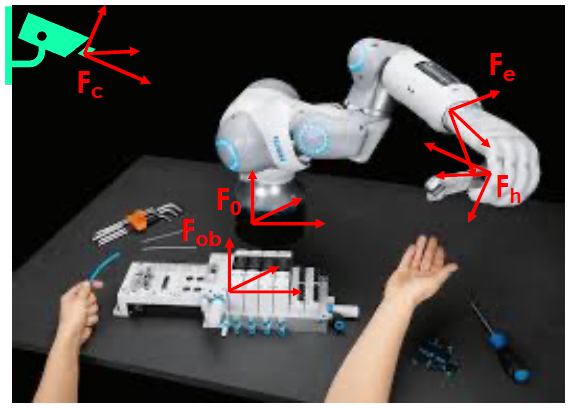
\includegraphics[width=0.65\linewidth]{imgs/homogeneous_workspace_robot.png}
  \caption{Frame transformations in a manipulation scenario (camera, robot, hand, object).}
\end{figure}

\hfill

\subsection{Homogeneous Transformations for Manipulators}

In the case of robotic manipulators, the pose of the end-effector (frame $F_n$) with respect to the robot base (frame $F_0$) depends on the configuration of the robot, specifically the values of the joint variables.

\paragraph{Direct (or Forward) Kinematics:}
It is the problem of determining the pose (position and orientation) of the end-effector given the joint variables. In other words, it computes the homogeneous transformation from base to end-effector:
\[
{}^0T_n = f(q_1, q_2, \dots, q_n)
\]
where $q_i$ are the joint variables (angles or displacements).

This is one of the \textbf{fundamental problems of robotics} and serves as the basis for motion planning, control, and simulation of robotic arms.

\begin{figure}[H]
  \centering
  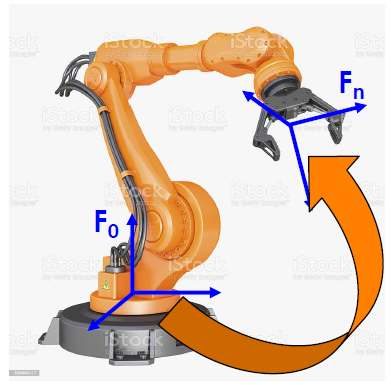
\includegraphics[width=0.4\linewidth]{imgs/forward_kinematics_robot_arm.png}
  \caption{Pose of the end-effector $F_n$ with respect to the robot base $F_0$, dependent on joint variables.}
\end{figure}

\hfill

\subsection{Forward Kinematics}

\paragraph{Definition:}
Forward kinematics (FK) consists in computing the pose of the end-effector of a manipulator given its configuration, i.e., the values of its joint variables. For an $n$-DOF robotic arm, this means:
\[
q \in \mathbb{R}^n \quad \Rightarrow \quad {}^0T_e(q) =
\begin{pmatrix}
{}^0R_e(q) & {}^0p_e(q) \\
\mathbf{0} & 1
\end{pmatrix}
\]

\paragraph{Key points:}
\begin{itemize}
  \item It allows to relate the joint variables (controlled inputs) to the pose of the end-effector (the part that interacts with the environment).
  \item It is crucial for understanding the movement of the end-effector resulting from joint actuation.
  \item It maps the \textbf{joint space} into the \textbf{task space}.
  \item The problem is \textbf{always solvable}, i.e., a unique pose can always be computed for a given configuration.
\end{itemize}

\paragraph{Solution method:}
Forward kinematics can be computed easily using the \textbf{Denavit-Hartenberg convention}, which systematically defines frame transformations along the links of a serial manipulator.

\hfill

\subsection{Inverse Kinematics}

\paragraph{Definition:}
Inverse kinematics (IK) is the problem of determining the joint configuration $q$ that produces a desired pose of the end-effector. Given:
\[
{}^0T_e = 
\begin{pmatrix}
{}^0R_e & {}^0p_e \\
\mathbf{0} & 1
\end{pmatrix}
\quad \Rightarrow \quad q = \text{IKINE}({}^0T_e)
\]

\paragraph{Importance:}
\begin{itemize}
  \item It is essential for converting motion specifications from the task space (e.g., Cartesian movements) into joint space commands that can be actuated by the robot.
  \item While forward kinematics is a direct computation, IK is often more challenging due to its mathematical structure.
\end{itemize}

\begin{figure}[H]
  \centering
  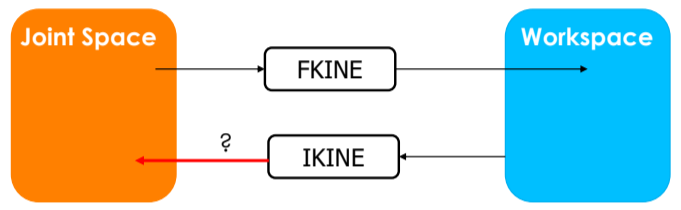
\includegraphics[width=0.6\linewidth]{imgs/ikine_mapping.png}
  \caption{Inverse kinematics maps the workspace pose back into the joint configuration space.}
\end{figure}

\paragraph{Challenges of Inverse Kinematics:}
\begin{itemize}
  \item IK equations are generally nonlinear.
  \item A closed-form solution may not always exist.
  \item There may be multiple or even infinite solutions (e.g., in redundant robots).
  \item Sometimes, no solution is admissible due to physical or kinematic constraints.
\end{itemize}

\begin{figure}[H]
  \centering
  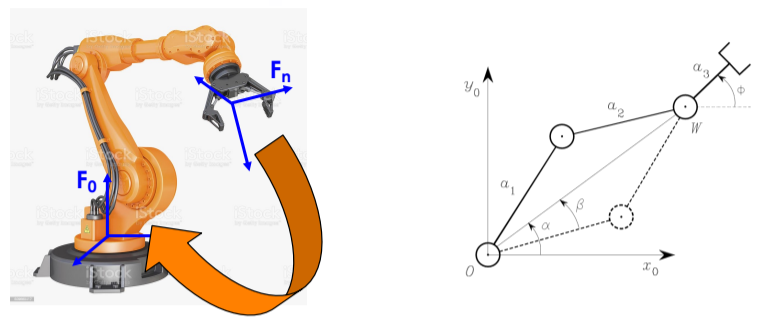
\includegraphics[width=0.8\linewidth]{imgs/ikine_robot_diagram.png}
  \caption{Example of a manipulator and schematic representation of link lengths and joint angles.}
\end{figure}

\paragraph{Solution Methods:}
\begin{itemize}
  \item \textbf{Closed-form}: Only possible in specific structures, usually using trigonometry or algebraic manipulation.
  \item \textbf{Numerical methods:} Needed when analytical solution is not feasible. Examples include:
  \begin{itemize}
    \item BFGS (Broyden-Fletcher-Goldfarb-Shannon)
    \item Levenberg–Marquardt
    \item Gradient projection methods
  \end{itemize}
  \item These methods minimize the error between the desired pose and the one obtained from the candidate solution.
\end{itemize}

\hfill

The direct and inverse kinematic problems are fundamental for describing the pose of the end-effector and the posture of the robot.

The composability of rotation matrices and of homogeneous transformation matrices is a very useful tool for representing the relative configurations between the robot(s) and other objects in the scene.

The Denavit–Hartenberg convention allows to have a standard for linking the joint configuration to the pose of the end-effector.

Inverse kinematics allows to map what happens in the workspace (e.g., specifications, desired poses), where no direct control is available, into the joint space, where it is possible to control the joints for achieving the desired behavior of the end-effector.

\hfill

Kinematics relates the configuration of the robot with the pose of the end-effector.

\begin{figure}[H]
    \centering
    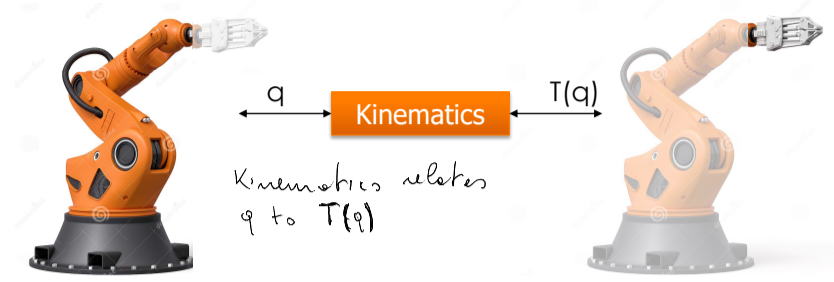
\includegraphics[width=1\linewidth]{imgs/differential_kinematics_begin.png}
\end{figure}

Kinematics relates the configuration of the robot in the joint space (determined by the joint variables) with the configuration of the end-effector in the workspace (determined, e.g., by homogeneous transformation matrix).

In order to map motions of the robot into motions of the end-effector and viceversa, it is important to relate velocities of the arm with velocities of the end-effector.

\hfill

\subsection{Differential Kinematics}

\paragraph{Def. 1:}

Consider a n-DOFs robotic arm. Given the speed of the joints, determine the linear and angular velocity of the end-effector.

It allows to map motions in the joint space into motions in the workspace.

It allows to understand how to move the joints in order to achieve a desired motion of the robot.

The relationship between joint velocities and the end-effector linear and angular velocity allows to characterize the mobility of the robot and to analyze its redundancy.

Given any representation of the pose of the end-effector (homogeneous matrix, etc.) with respect to a given frame (e.g., the base frame), the \textbf{velocity of the end-effector} can be represented by a 3-dimensional translational velocity and by a 3-dimensional angular velocity. \textit{Note:} This is called \textbf{Twist}.
  
The problem addressed by differential kinematics is to find a relation between the speed of the joints and the linear and angular velocity of the end-effector.

\textbf{Def. 2:} Consider a n-DOFs robotic arm, where $q = (q_1, \dots, q_n)^T$ is the joint vector. Express the linear and angular velocities of the end-effector $\dot{p}_e$ and $\omega_e$ as a function of the joint speed $\dot{q} = (\dot{q}_1, \dots, \dot{q}_n)^T$.

The sought relations are both linear in the joint velocities, which means:

\[
\dot{p}_e = J_P(q) \dot{q}
\]
\[
\omega_e = J_O(q) \dot{q}
\]

$\mathbf{J_P(q)}$: $(3 \times n)$ matrix relating the contribution of the joint velocities to the end-effector linear velocity $\dot{p}_e$.

$\mathbf{J_O(q)}$: $(3 \times n)$ matrix relating the contribution of the joint velocities to the end-effector angular velocity $\omega_e$.

In compact form, these relations can be written as:

\[
v_e = 
\begin{bmatrix}
\dot{p}_e \\
\omega_e
\end{bmatrix}
= J(q) \dot{q}
\quad\text{(6-dimensional vector)}
\]

This represents the manipulator \textbf{differential kinematics} equation, and the vector $v_e$ is called \textbf{generalized velocity} or \textbf{twist} of the end-effector.

The $6 \times n$ matrix $J(q)$ is the \textbf{geometric Jacobian} of the robot, where $n$ is the number of DOFs:
  \[
  J(q) = 
  \begin{pmatrix}
  J_P(q) \\
  J_O(q)
  \end{pmatrix}
  \]

In general, it depends on the joint variables.
  
It is possible to write:

\[
  J(q) =
  \begin{pmatrix}
  J_{P_1} & \dots & J_{P_n} \\
  J_{O_1} & \dots & J_{O_n}
  \end{pmatrix}
\]

whence:

\[
  J(q) \dot{q} =
  \begin{pmatrix}
  J_{P_1} \\
  J_{O_1}
  \end{pmatrix} \dot{q}_1 +
  \begin{pmatrix}
  J_{P_2} \\
  J_{O_2}
  \end{pmatrix} \dot{q}_2 + \dots +
  \begin{pmatrix}
  J_{P_n} \\
  J_{O_n}
  \end{pmatrix} \dot{q}_n
\]
  
\textit{Note (handwritten annotation):} In the case of two vectors, these sums indicate that we can move with velocities $\dot{q}_1$ and $\dot{q}_2$ along the directions defined by the respective vectors $\begin{pmatrix} J_{P_1} \\ J_{O_1} \end{pmatrix}$ and $\begin{pmatrix} J_{P_2} \\ J_{O_2} \end{pmatrix}$, i.e. on a plane.

The structure of each joint determines how the corresponding joint speed contributes to the twist.

\hfill

\paragraph{Kinematic Singularities} \hfill

The differential kinematics provides a linear relation between the twist of the end-effector $v_e$ and the joint velocities $\dot{q}$:
\[
v_e = J(q) \dot{q}
\]
\textit{Nota (annotazione a penna):} In pratica, la Jacobiana $J(q)$ ci dice quali movimenti può o non può eseguire il robot.

The configurations where $J(q)$ is \textbf{rank deficient} are termed \textbf{kinematic singularities}.
\textit{Nota (annotazione a penna):} Quando $J$ è rank-deficient, significa che manca il contributo di una colonna (perché è combinazione lineare di un'altra), ovvero alcune direzioni di movimento non possono essere raggiunte dal robot.

To find the singularities of a manipulator is of great interest for the following reasons:
\begin{itemize}
    \item Singularities represent configurations at which mobility of the structure is reduced, i.e., it is not possible to impose an arbitrary motion to the end-effector.
    \item When the structure is at a singularity, infinite solutions to the inverse kinematics problem may exist.
    \item In the neighbourhood of a singularity, small velocities in the operational space may cause large velocities in the joint space.
\end{itemize}

When the robot is in a singularity configuration, no value of joint velocities $\dot{q}$ exists for moving the end-effector in some direction.

\begin{figure}[H]
    \centering
    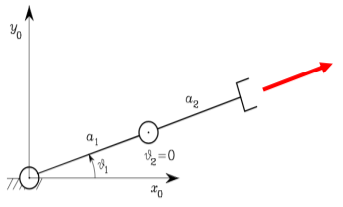
\includegraphics[width=0.6\linewidth]{imgs/kinematic_sing_1.png}
\end{figure}

If a robot has 6 DOFs, the Jacobian is square and the rank deficient configurations are those where:
\[
\det(J(q)) = 0
\]

Thus, all the kinematic singularities can be found by solving the algebraic equation $\det(J(q)) = 0$ in $q$.

\begin{itemize}
    \item The equation $\det(J(q)) = 0$ is very nonlinear and a numerical solver may be used for solving it.
\end{itemize}

They can be classified into:

\textbf{Boundary singularities:} occur when the manipulator is either out-stretched or retracted. They are easy to avoid by keeping the robot far from the boundary of its workspace.

\begin{figure}[H]
    \centering
    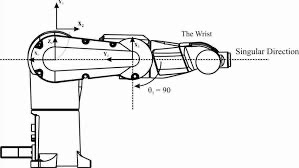
\includegraphics[width=0.6\linewidth]{imgs/boundary_singularity.png}
    \caption{Example of a boundary singularity when the manipulator is fully extended.}
\end{figure}

\textbf{Internal singularities:} occur inside the reachable workspace and are generally caused by the alignment of two or more axes of motion, or by the attainment of particular end-effector configurations. They are hard to avoid.

\begin{figure}[H]
    \centering
    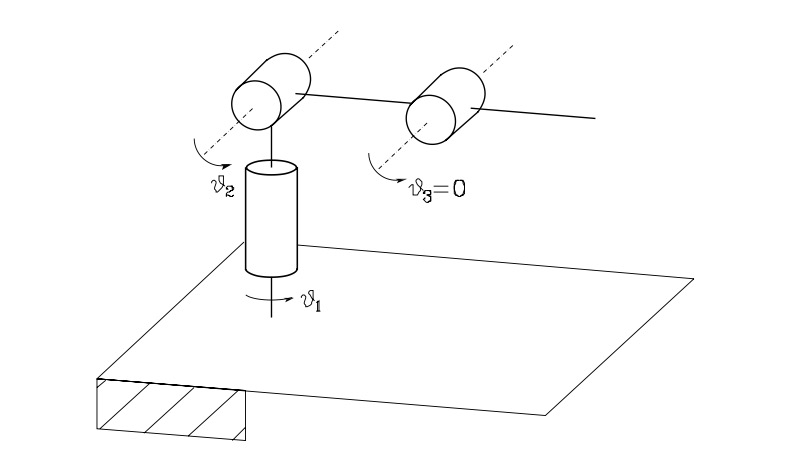
\includegraphics[width=0.6\linewidth]{imgs/internal_singularity.png}
    \caption{Example of an internal singularity due to axis alignment.}
\end{figure}

\hfill

\subsection{Inverse Differential Kinematics}

\textbf{Def.:} Consider a n-DOFs robotic arm, where $q = (q_1, \dots, q_n)^T$ is the joint vector. Given a desired twist $v_e$ for the end-effector, find the joint velocities that produce $v_e$.

This is a very important problem to be solved (often online) for finding the speed to control the joints for moving the end-effector with the desired twist $v_e$.

Thanks to the linear relation of the differential kinematics:

\[
    v_e = J(q) \dot{q}
\]

the inverse differential kinematics is much easier to address than inverse kinematics.

If $n = m$, i.e., the dimension of the joint space is the same as the one of the workspace, the Jacobian is square and the inverse differential kinematics problem can be solved by:

\[
    \dot{q} = J^{-1}(q) v_e
\]

If the Jacobian is \textbf{NOT} invertible, i.e., if $\det(J(q)) = 0$, the robot is in a singular configuration. Its mobility is limited and the inverse differential kinematics cannot be solved.

\textit{Nota (annotazione a penna):} Può accadere che la Jacobiana non sia invertibile perché essa non è una matrice costante, dato che dipende dalla configurazione degli angoli del robot.

It is necessary to plan the motion of the robot to keep it away from singular configurations. In this way, it is always possible to compute the motion of the joints to reproduce the desired motion of the end-effector.

If $n > m$, i.e., if the robot is redundant, the Jacobian is rectangular and the inverse does not exist.

If the Jacobian has full rank, then the inverse differential kinematics problem admits \textbf{infinitely many solutions}.

It is possible to exploit the concept of \textbf{pseudo-inverse of the Jacobian} for selecting a specific solution:

\[
\dot{q} = J^{+}(q) v_e
\quad\text{where}\quad
J^{+} = J^T (J J^T)^{-1}
\]

\textit{Nota (annotazione a penna):} $J^{+}$ is the pseudo-inverse.

In this case $\dot{q}$ is the minimum norm solution to the inverse differential kinematics problem. This means that:

\[
\|\dot{q}\| = \sqrt{\dot{q}_1^2 + \cdots + \dot{q}_n^2}
\]

is minimal, i.e. the pseudo inverse finds the lowest speed solution.

\textit{Nota (annotazione a penna):} Minore è la velocità, meglio è: minor sforzo sui motori e minor dispendio energetico.

\begin{figure}[H]
    \centering
    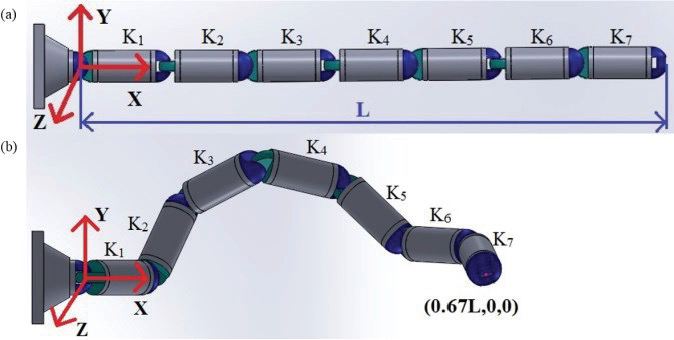
\includegraphics[width=1\linewidth]{imgs/inverse_diff_kine.png}
\end{figure}

Infinitely many joint speeds can instantaneously move the robot along a desired direction.

The pseudo inverse of the Jacobian exists only if the Jacobian is full rank. Thus, if the Jacobian is not full rank, the robot loses mobility and the inverse differential kinematics cannot be solved.

It is necessary to plan the motion of the robot to keep it away from singular configurations. In this way, it is always possible to compute the motion of the joints to reproduce the desired motion of the end-effector.

\textit{Nota (annotazione a penna):} Da una determinata velocità lineare posso ottenere la corrispondente velocità angolare:

\begin{figure}[H]
    \centering
    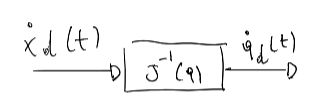
\includegraphics[width=0.4\linewidth]{imgs/inv_diff_kine_speeds.png}
\end{figure}

\[
J^{-1}(q) = \frac{1}{\det(J(q))} \, A^{T}
\]

$\det(J(q))$ is a continuous function.

\subsubsection*{Analytical Jacobian}

The Jacobian we saw before was geometric.

If the end-effector pose is specified in terms of a minimal number of parameters in the operational space, it is natural to compute the Jacobian via differentiation of the direct kinematics function with respect to the joint variables.

The translational velocity of the end-effector frame can be expressed as the time derivative of vector $\mathbf{p}_e$ representing the origin of the end-effector frame with respect to the base frame, i.e.,
    
\[
    \dot{\mathbf{p}}_e = \frac{\partial \mathbf{p}_e}{\partial \mathbf{q}} \dot{\mathbf{q}} = J_P(\mathbf{q}) \dot{\mathbf{q}}
\]

For what concerns the rotational velocity of the end-effector frame, the minimal representation of orientation in terms of three variables $\boldsymbol{\phi}_e$ can be considered. \textcolor{red}{Its time derivative in general differs from the angular velocity vector previously defined}.

\[
    \dot{\boldsymbol{\phi}}_e = \frac{\partial \boldsymbol{\phi}_e}{\partial \mathbf{q}} \dot{\mathbf{q}} = J_{\phi}(\mathbf{q}) \dot{\mathbf{q}}
\]

Upon these premises, the \textbf{differential kinematics equation} can be obtained as the time derivative of the direct kinematics equation, i.e.:

\[
\dot{x}_e =
\begin{bmatrix}
\dot{p}_e \\
\dot{\phi}_e
\end{bmatrix}
=
\begin{bmatrix}
J_P(q) \\
J_\phi(q)
\end{bmatrix}
\dot{q}
= J_A(q)\dot{q}
\]

where the \textbf{analytical Jacobian}

\[
J_A(q) = \frac{\partial k(q)}{\partial q}
\]

is different from the geometric Jacobian $J(q)$ since the end-effector angular velocity $\boldsymbol{\omega}_e$ with respect to the base frame is not given by $\dot{\phi}_e$.

It is possible to find the relationship between the angular velocity $\boldsymbol{\omega}_e$ and the rotational velocity $\dot{\phi}_e$ for a given set of orientation angles.

Equation relating the angular velocity to the time derivative of the Euler angles:

\[
\boldsymbol{\omega}_e = T(\phi_e)\dot{\phi}_e, \quad
T =
\begin{bmatrix}
0 & -\sin \varphi & \cos \varphi \, \sin \vartheta \\
0 & \cos \varphi & \sin \varphi \, \sin \vartheta \\
1 & 0 & \cos \vartheta
\end{bmatrix}.
\]

Once the transformation $T$ between $\boldsymbol{\omega}_e$ and $\dot{\phi}_e$ is given, the analytical Jacobian can be related to the geometric Jacobian as:

\[
\boldsymbol{v}_e =
\begin{bmatrix}
I & 0 \\
0 & T(\phi_e)
\end{bmatrix}
\dot{x}_e
= T_A(\phi_e)\dot{x}_e
\]

\[
J = T_A(\phi) J_A
\]

This relationship shows that $J$ and $J_A$, in general, differ.

The Analytical Jacobian is often used in control schemes. In fact, a minimal representation of the twist can be integrated for achieving the pose of the end-effector. This cannot be achieved using the geometric Jacobian since the integral of the angular velocity \textbf{is not} the orientation of the end-effector.

\[
\dot{q} \;\; \xrightarrow{\;\; J(q) \;\;} \;\; 
v_e = 
\begin{pmatrix}
\dot{p}_e \\ 
\omega_e
\end{pmatrix}
\;\; \xrightarrow{\;\; \int \;\;} \;\;
x_e = 
\begin{pmatrix}
p_e \\ 
\times
\end{pmatrix}
\quad \text{to control (wrong)}
\]

\begin{figure}[H]
    \centering
    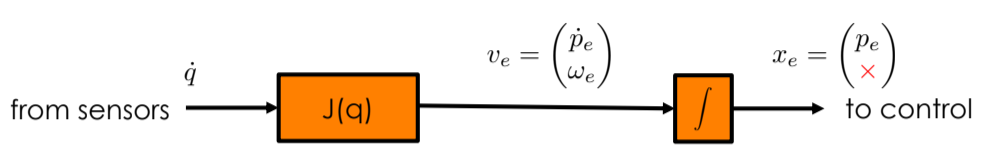
\includegraphics[width=0.85\linewidth]{imgs/diff_kine_1.png}
\end{figure}

\[
\dot{q} \;\; \xrightarrow{\;\; J_A(q) \;\;} \;\; 
v_e = 
\begin{pmatrix}
\dot{p}_e \\ 
\dot{\phi}_e
\end{pmatrix}
\;\; \xrightarrow{\;\; \int \;\;} \;\;
x_e = 
\begin{pmatrix}
p_e \\ 
\phi_e
\end{pmatrix}
\quad \text{to control (correct)}
\]

\begin{figure}[H]
    \centering
    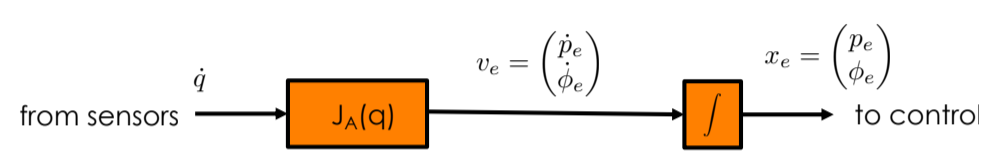
\includegraphics[width=0.85\linewidth]{imgs/diff_kine_2.png}
\end{figure}

\subsection{Statics}

\textbf{Def:} Consider a n-DOFs robotic arm. Given the force and the torque applied to the end-effector, determine the corresponding torques/forces applied to the joints.

It allows to map interactions in the workspace into actions on the joint space.

It allows to understand how to control the joints in order to achieve a desired interaction of the robot with the environment.

Let $\boldsymbol{\tau}$ denote the $(n \times 1)$ vector of joint torques/forces and $\boldsymbol{w}_e$ the $(6 \times 1)$ vector of generalized force, also called \textbf{wrench}, applied to the end-effector. 

The wrench has the following structure:

\[
\boldsymbol{w}_e =
\begin{pmatrix}
\boldsymbol{f}_e \\
\boldsymbol{\mu}_e
\end{pmatrix}, 
\qquad \boldsymbol{f}_e \in \mathbb{R}^3, \quad 
\boldsymbol{\mu}_e \in \mathbb{R}^3
\]

where $\boldsymbol{f}_e$ and $\boldsymbol{\mu}_e$ are the force and the torque applied to the end-effector.

The application of the \textit{principle of virtual work} allows the determination of the required relationship that can be summarized as:

\[
\boldsymbol{\tau} = J^T(q)\boldsymbol{w}_e
\]

stating that the relationship between the end-effector forces and the joint torques is established by the transpose of the manipulator geometric Jacobian.

\hfill

\subsection{Recap on Kinematics Relationship and Differential Kinematics}

\begin{figure}[H]
    \centering
    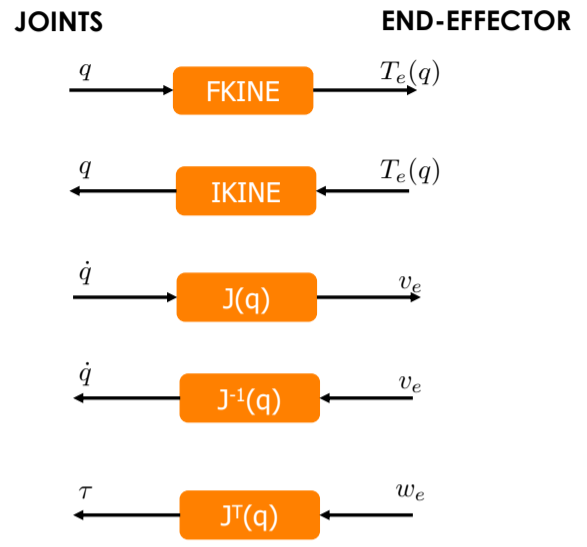
\includegraphics[width=0.65\linewidth]{imgs/kinematic_relationship.png}
    \caption{Kinematics Relationship}
\end{figure}

Differential kinematics and inverse differential kinematics are fundamental for mapping the motion of the robot into the motion of the end-effector and viceversa.
    
The Jacobian matrix is a fundamental object, describing the mobility of the end-effector.
    
Singularity configurations are points where the robot loses mobility in one or more directions.
    
The Jacobian allows to map wrenches applied to the end-effector into equivalent torques on the joints.

\hfill

Kinematics allows to capture the configuration of the robot and the pose of the end-effector.
    
In order to capture information about the behavior of the robot under the effect of external forces (e.g. gravity, wrenches on the end-effector, torques/forces on the joint), it is necessary to build a dynamic model of the manipulator.
    
The most common and useful strategy for building the dynamic model is the Euler-Lagrange formulation, that generalizes the second Newton law to multi-body systems.

\hfill

\subsection{Dynamics}

Joints can be actuated by linear forces (prismatic joints) or by torques (revolute joints).
    
The set of torques/linear forces is grouped in a vector $\tau \in \mathbb{R}^n$.

By applying a force/torque to the joints it is possible to change the configuration of the robot and, consequently, the pose of the end-effector.
    
Force/torques on the joints and external wrenches applied on the end-effector are the external action applied on the robot and that produce a motion of the overall structure.

\hfill

\subsection{Dynamic model in the joint space}

\textbf{Def:} Consider a n-DOFs robotic arm. Build the dynamic relation between the torques/forces acting on joints and the acceleration of the joints.

It allows to understand the effect of forces/torques on the joints on the motion of the robot.
    
It is the model that will be used for controlling the motion of the robot in the joint space.
    
The model can be built exploiting the Lagrangian formulation.

Using the Lagrangian formalism, the mechanics of the multi-body robotic arm leads to the following model:

\[
    M(q)\ddot{q} + C(q, \dot{q})\dot{q} + g(q) = \tau
\]

Joints can be affected by dynamic friction, due to the non-idealities in the coupling. Furthermore, an external wrench acting on the end-effector can produce extra torques acting on the robot. These effects can be modeled by adding external actions as:

\[
    M(q)\ddot{q} + C(q, \dot{q})\dot{q} + g(q) = \tau - D\dot{q} + J^T(q)w_e
\]

Usually the terms related to the physics of the robot are on the same side and the \textbf{Euler-Lagrange model in the joint space} is written as

\[
    M(q)\ddot{q} + C(q, \dot{q})\dot{q} + D\dot{q} + g(q) = \tau + J^T(q)w_e
\]

\hfill

\subsection{Properties of the Euler-Lagrange model}

$M(q)$ is a square, symmetric and positive definite matrix

\[
    M^T(q) = M(q), \qquad x^T M(q) x > 0 \quad \forall x \neq 0, \; x \in \mathbb{R}^n
\]  

This is the \textit{inertia}.

$D$ is a square, (usually) symmetric and positive definite matrix

\[
    D^T = D, \qquad x^T D x > 0 \quad \forall x \neq 0, \; x \in \mathbb{R}^n
\]  

This is the \textit{friction on all the joints}.  

The matrix $\dot{M}(q) - 2C(q,\dot{q})$ is \textbf{skew-symmetric} ($A^T = -A$)  

\[
    (\dot{M}(q) - 2C(q,\dot{q}))^T = -(\dot{M}(q) - 2C(q,\dot{q}))
\]  

\[
    x^T (\dot{M}(q) - 2C(q,\dot{q})) x = 0 \quad \forall x \neq 0, \; x \in \mathbb{R}^n
\]  

\hfill

To recap, the terms of the Euler--Lagrange model can be summarized as follows:

\begin{itemize}
    \item $\mathbf{M(q)}$: inertia matrix, square, symmetric and positive definite.
    \item $\mathbf{C(q,\dot{q})\dot{q}}$: Coriolis and centrifugal terms.
    \item $\mathbf{D\dot{q}}$: viscous friction and joint dissipative effects.
    \item $\mathbf{g(q)}$: gravity terms acting on the manipulator.
    \item $\mathbf{\tau}$: vector of joint torques/forces.
    \item $\mathbf{J^T(q)w_e}$: contribution of external forces (wrench) mapped to the joints through the Jacobian transpose.
\end{itemize}

\hfill

\subsection{Dynamic Model in the task space}

The dynamic model of the robot can be formulated also in the task space. This is useful for modeling the dynamic behavior of the end-effector.  

The dynamic model in the task space can be derived starting from the dynamic model in the joint space.  

The most common formulation of the dynamic model in the task space represents the pose of the end-effector as a $6 \times 1$ vector, using Euler angles for representing the pose.

The \textbf{dynamic model in the task space} is given by:
\[
    M_A(x_e)\ddot{x}_e + C_A(x_e, \dot{x}_e)\dot{x}_e + D_A\dot{x}_e + g_A(x_e) = w_d + w_f
\]

where:
\[
    M_A(x_e) = \left(J_A M^{-1} J_A^T \right)^{-1}
\]
\[
    C_A(x_e, \dot{x}_e)\dot{x}_e = J_A^{-T} C \dot{q} - M_A \dot{J}_A \dot{q}
\]
\[
    D_A = J_A^{-T} D
\]
\[
    g_A = J_A^{-T} g
\]

\hfill

The dynamic model in the task space enjoys the same properties as the dynamic model in the joint space.  

Unlike the dynamic model in the joint space, the dynamic model in the task space is well defined when the robot is not close to singularities.  

\newpage